\begin{frame}{Wybór obserwacji}
	
	\begin{columns}
		\begin{column}{.8\hsize}
			\textbf{Obserwacje:}
			\begin{itemize}
				\myitem dane pobrane bezpośrednio z równania trasy
				\myitem dane odległości od krawędzi
				\myitem dane wizualne jednowymiarowe
				\myitem dane wizualne z kamery przedniej
				\myitem dane wizualne z kamery z lotu ptaka
			\end{itemize}
			\vspace{5mm}
		\end{column}
		
		\begin{column}{.2\hsize}
			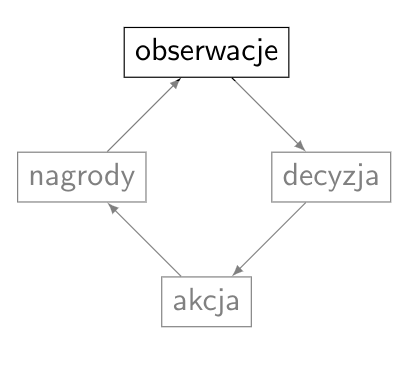
\includegraphics[width=\linewidth]{figures/learning_loop_1.png}
			\vspace{15mm}
		\end{column}
	\end{columns}

	\begin{columns}
		\begin{column}{.3\hsize}
			\hspace*{3.9cm}
			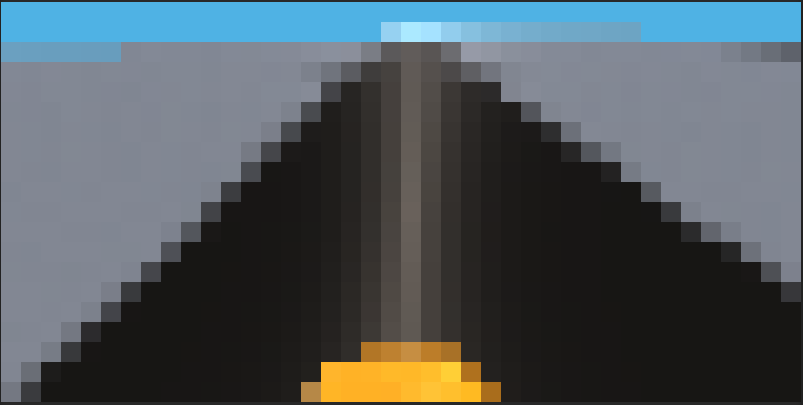
\includegraphics[width=\linewidth]{figures/observations_2.png}
		\end{column}
	\end{columns}

	\begin{columns}
		\begin{column}{.3\hsize}
			\centering
			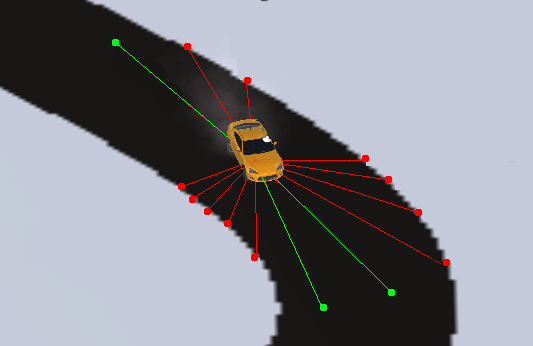
\includegraphics[width=\linewidth]{figures/observations_0.png}
		\end{column}
		\begin{column}{.3\hsize}
			\centering
			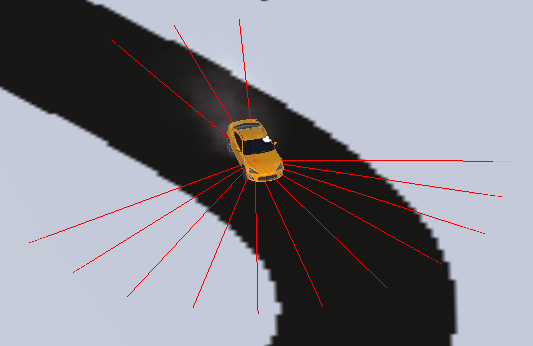
\includegraphics[width=\linewidth]{figures/observations_1.png}
		\end{column}
		\begin{column}{.3\hsize}
			\centering
			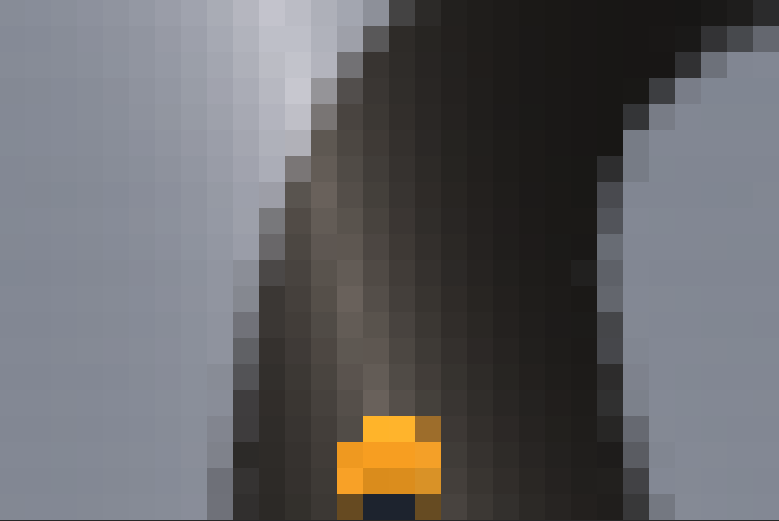
\includegraphics[width=\linewidth]{figures/observations_3.png}
		\end{column}
	\end{columns}
	
\end{frame}
